 % !TEX encoding = UTF-8 Unicode
\documentclass[11pt]{article}

\usepackage[a4paper]{geometry}
\geometry{verbose,tmargin=2.5cm,bmargin=2cm,lmargin=2cm,rmargin=2cm} %Vodorovná čára nahoře na stránce
\usepackage{fancyhdr}

\pagestyle{fancy}
%\pagestyle{headings}

%nastavení písma a češtiny
\usepackage[english, czech]{babel}
\usepackage[T1]{fontenc} % pouzije EC fonty 
\usepackage[utf8]{inputenc} % pro unicode UTF-8

% odkazy
\usepackage{url}

% vícesloupkové tabulky
\usepackage{multirow}
\usepackage{multicol}

% vnoření popisu obrázků
\usepackage{subcaption}

% automatickб konverze EPS 
\usepackage{graphicx} 
\usepackage{epstopdf}

%indexi a rejstřík
\usepackage{index}

% odkazy a zбloћky
\usepackage[unicode=true, bookmarks=true,bookmarksnumbered=true,
bookmarksopen=false, breaklinks=false,pdfborder={0 0 0},
pdfpagemode=UseNone,backref=false,colorlinks=false] {hyperref}

% Poznбmky při překladu
\usepackage{xkeyval}	% Inline todonotes
\usepackage[textsize = footnotesize]{todonotes}
\presetkeys{todonotes}{inline}{}

%Řádkování
\usepackage{setspace}
%Použiti
%\onehalfspacing
%\singlespacing
%\onehalfspacing
%\setstretch{1.1}

\setlength\parindent{0pt}

% Zacni sekci slovem ukol
\renewcommand{\thesection}{}
% enumerate zacina s pismenem
%\renewcommand{\theenumi}{ \alph{enumi}}

%Akord makro
\newcommand{\ch}[1]
{
    \makebox[-6pt][c]{\raisebox{12pt}[24pt]{~~{ \footnotesize \textbf{#1}} }}
}

\newcounter{sloka}
\setcounter{sloka}{2}
\newcommand{\vloz}[1]{\include{#1} \setcounter{sloka}{2}}

\newcommand{\sloka}{\textbf{Sloka \arabic{sloka}} \refstepcounter{sloka} \\*}
\newcommand{\refren}{\textbf{Refrén:}\\*}
\newcommand{\refrenSecond}{\textbf{Refrén 2:}\\*}


%indexi
\newindex{author}{adx}{and}{Autoři}
\def\aindex{\index[author]}


\fancyhf{}

% zahlavi
\usepackage{titling}
\fancyhf[HC]{\thetitle}
\fancyhf[HLE,HRO]{\theauthor}
%\fancyhf[HRE,HLO]{\today}
%zapati
\fancyhf[FLE,FRO]{\thepage}

\makeatother

%Údaje o autorovy
\title{Vodácký zpěvník}
\author{Pohodičkáři}
\date{\today} 

%Grafika akordů
\usepackage{gchords}

\begin{document}
\maketitle

\begin{figure}[htbp]
  \centering
  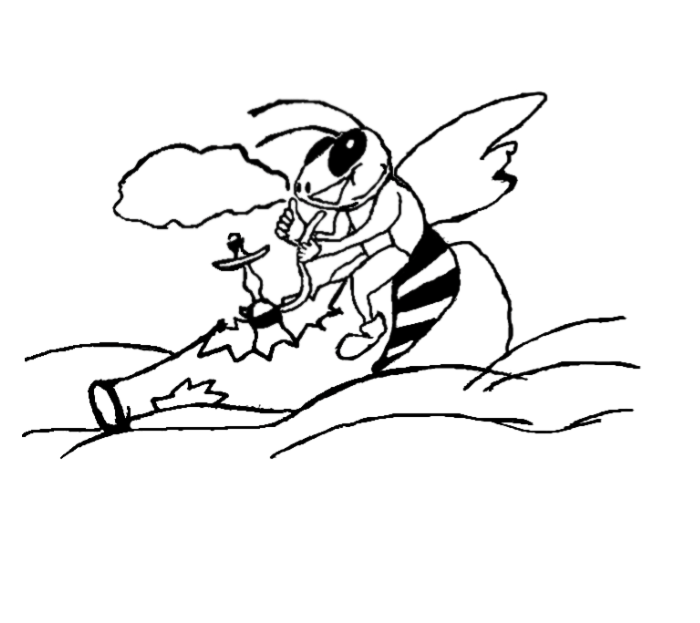
\includegraphics[width=16cm]{img/main_img2.png}
  %\caption{Magický trojúhelník se čtyřmi vnitřními úhly a pěti stranami.}
\end{figure}

\newpage

\begin{multicols}{2}
\tableofcontents % vytvoří obsah podle souboru priklad.toc
\newpage % provede odstránkování
\end{multicols}

\printindex[author] % vytvoří obsah podle souboru priklad.toc
% terminal příkaz: makeindex -o Zpevnik.and Zpevnik.adx

\section*{Akordy}
%\smallchords

%C
\renewcommand{\C}{\chord{t}{n,p3,p2,n,p1,n}{C}} 

%D
\newcommand{\D}{\chord{t}{x,n,n,p2,p3,p2}{D}} 

%E
\newcommand{\E}{\chord{t}{n,p2,p2,p1,n,n}{E}} 

%F
\newcommand{\F}{\chord{t}{x,n,p3,p2,p1,p1}{F}} %TODO vlnka přes p1

%A
\newcommand{\A}{\chord{t}{n,n,p2,p2,p2,n}{A}} 

%H 
%\newcommand{\H}{\chord{t}{n,n,p2,p2,p2,n}{A}} %chybí

%G
\renewcommand{\G}{\chord{t}{p3,p2,n,n,n,p3}{G}} 

%B
\newcommand{\B}{\chord{t}{x,x,p4,p4,p4,p2}{B}} 

%------------------------------------------------------
%C7
\newcommand{\Cseven}{\chord{t}{n,p3,p2,p3,p1,n}{C7}} 

%D7
\newcommand{\Dseven}{\chord{t}{n,n,n,p2,p1,p2}{D7}} 

%E7
\newcommand{\Eseven}{\chord{t}{n,p2,p2,p1,p3,n}{E7}} 

%G7
\newcommand{\Gseven}{\chord{t}{p3,p2,n,n,n,p1}{G7}} 

%A7
\newcommand{\Aseven}{\chord{t}{n,n,p2,n,p2,n}{A7}}

%F7
\newcommand{\Fseven}{\chord{t}{x,x,p1,p2,p1,p1}{F7}}  %TODO vlna pře krajní F7

%B7
\newcommand{\Bseven}{\chord{t}{x,p2,p1,p2,n,p2}{B7}} 

%------------------------------------------------------
%Cm
\newcommand{\Cm}{\chord{t}{x,x,p5,p5,p4,p3}{Cmi}} 

%Dm
\newcommand{\Dm}{\chord{t}{x,x,n,p2,p3,p1}{Dmi}} 

%Em
\newcommand{\Em}{\chord{t}{n,p2,p2,n,n,n}{Emi}} 

%Gm
\newcommand{\Gm}{\chord{t}{n,n,p5,p3,p3,p3}{Gmi}} %TODO Vlnka přes p3

%Am
\newcommand{\Am}{\chord{t}{x,n,p2,p2,p1,n}{Ami}}

%F
\newcommand{\Fm}{\chord{t}{x,x,p3,p1,p1,p1}{Fmi}} %TODO vlnka přes p1 

%B
\newcommand{\Bm}{\chord{t}{x,x,p4,p4,p3,p2}{Bm}} 

%------------------------------------------------------
%C7+
\newcommand{\CsevenPlus}{\chord{t}{n,p3,p2,p3,p1,n}{C7}} 


%A7+
\newcommand{\AsevenPlus}{\chord{t}{x,n,p2,p1,p2,n}{A7+}} 

$$
\begin{array}{ccccccc}
\upchord{\C} \qquad \qquad & \upchord{\D} \qquad \qquad& \upchord{\E} \qquad \qquad& \upchord{\G}  \qquad \qquad& \upchord{\A} \qquad \qquad& \upchord{\F}  \qquad \qquad & \upchord{\B}  \qquad \qquad \\
\upchord{\Cseven} \qquad \qquad & \upchord{\Dseven} \qquad \qquad& \upchord{\Eseven} \qquad \qquad& \upchord{\Gseven}  \qquad \qquad& \upchord{\Aseven} \qquad \qquad& \upchord{\Fseven}  \qquad \qquad & \upchord{\Bseven}  \qquad \qquad \\
\upchord{\Cm}\qquad \qquad & \upchord{\Dm} \qquad \qquad& \upchord{\Em} \qquad \qquad&  \upchord{\Gm} \qquad \qquad& \upchord{\Am} \qquad \qquad& \upchord{\Fm}  \qquad \qquad & \upchord{\Bm}  \qquad \qquad \\


\end{array} 
$$


\newpage

%Pisničky
%-------------------------------------------------
\vloz{songs/1970}
\vloz{songs/1Signalni}
\vloz{songs/Amerika}
\vloz{songs/Andel}
\vloz{songs/Batalion}
\vloz{songs/BednaOdWhisky}
\vloz{songs/BlaznovaUkolebavka}
\vloz{songs/Buraky}
\vloz{songs/CerniAndele}
\vloz{songs/Cesta}
\vloz{songs/Davno}
\vloz{songs/DivokyKone}
\vloz{songs/DlouhejKour}
\vloz{songs/DobrakOdKosti}
\vloz{songs/DrobnaParalela}
\vloz{songs/FrankyDlouhan}
\vloz{songs/HejCloveceBozi}
\vloz{songs/HlidacKrav}
\vloz{songs/HolubiDum}
\vloz{songs/JahodyMrazeny}
\vloz{songs/KdyzMeBraliZaVojaka}
\vloz{songs/KdyzNasTataHral}
\vloz{songs/Kometa}
\vloz{songs/Kozel}
\vloz{songs/NahrobniKamen}
\vloz{songs/Okor}
\vloz{songs/Panenka}
\vloz{songs/PojdmeSeNapit}
\vloz{songs/RanaVTrave}
\vloz{songs/RekniKdeTyKytkyJsou}
\vloz{songs/Riptide}
\vloz{songs/SeverniVitr}
\vloz{songs/SlaviciZMadridu}
\vloz{songs/SlzyTvyMamy}
\vloz{songs/StaraArcha}
\vloz{songs/TisicMil}
\vloz{songs/TrajdaCopata}
\vloz{songs/TriKrize}
\vloz{songs/VedMeDalCestoMa}
\vloz{songs/WishYouWereHere}
\vloz{songs/Zafukane}
\vloz{songs/ZahradaTicha}
\vloz{songs/Zatanci}
\vloz{songs/ZatracenejZivot}
\vloz{songs/Zelva}
\vloz{songs/Zuzana}

\vloz{songs/VltavaTOUR}
\vloz{songs/OhreTOUR}

\end{document}